%%%%%%%%%%%%%%%%%%%%%%%%%%%%%%%%%%%%%%%%%%%%%%%%%%%%%%%%%%%%%%%%%%%%%
% LaTeX Template: Project Titlepage Modified (v 0.1) by rcx
%
% Original Source: http://www.howtotex.com
% Date: February 2014
% 
% This is a title page template which be used for articles & reports.
% 
% This is the modified version of the original Latex template from
% aforementioned website.
% 
%%%%%%%%%%%%%%%%%%%%%%%%%%%%%%%%%%%%%%%%%%%%%%%%%%%%%%%%%%%%%%%%%%%%%%

\documentclass[12pt]{report}
\usepackage[a4paper]{geometry}
\usepackage[myheadings]{fullpage}
\usepackage{fancyhdr}
\usepackage{lastpage}
\usepackage{graphicx, wrapfig, subcaption, setspace, booktabs, hyperref}
\usepackage[T1]{fontenc}
\usepackage[font=small, labelfont=bf]{caption}
\usepackage{fourier}
\usepackage[protrusion=true, expansion=true]{microtype}
\usepackage[english]{babel}
\usepackage{sectsty}
\usepackage{url, lipsum}


\newcommand{\HRule}[1]{\rule{\linewidth}{#1}}
\onehalfspacing
\setcounter{tocdepth}{5}
\setcounter{secnumdepth}{5}

%-------------------------------------------------------------------------------
% HEADER & FOOTER
%-------------------------------------------------------------------------------
\pagestyle{fancy}
\fancyhf{}
\setlength\headheight{15pt}

\fancyfoot[R]{Page \thepage\ of \pageref{LastPage}}
%-------------------------------------------------------------------------------
% TITLE PAGE
%-------------------------------------------------------------------------------

\begin{document}

\title{ \normalsize \textsc{}
		\\ [2.0cm]
		\HRule{0.5pt} \\
		\LARGE \textbf{\uppercase{Trading Post Problem}}
		\HRule{2pt} \\ [0.5cm]
		\normalsize \today \vspace*{5\baselineskip}}

\date{}

\author{
		 \\ 
		Jake McKenzie, Joseph Musngi, and Matthew Skipworth \\ \\
		Design And Analysis Of Algorithms }

\maketitle
\tableofcontents

\newpage

%-------------------------------------------------------------------------------
% Section title formatting
%\section*{Contents}
\sectionfont{\scshape}
%-------------------------------------------------------------------------------

%-------------------------------------------------------------------------------
% BODY
%-------------------------------------------------------------------------------

\section*{Problem Statement}
\addcontentsline{toc}{section}{Problem Statement}
There are \textit{n} trading posts numbered 1 to \textit{n}, as you travel 
downstream. At any trading post \textit{i}, you can rent a canoe to be returned 
at any of the downstream posts$i>i$. You are given a cost array $R(i,j)$ giving 
the cost of these rentals for $1 \leq i \leq j \leq n$. We will have to assume 
that $R(i,i)=0$ and $R(i,j)=\infty$ if $i>j$. For example, with $n=4$, the cost 
array may look as follows: The rows are the sources $(i-s)$ and the columns 
are the destinations $(j's)$.$$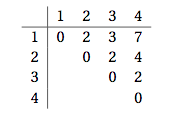
\includegraphics[scale=.8]{image1.png}$$ The 
problem is to find a solution that computes the cheapest sequence of rentals 
taking you from post 1 all the way to post \textit{n}. In this example, the 
cheapest sequence is to rent form post 1 to post 3 (cost 3), then from post 3 
to post 4 (cost 2), with a total cost of 5 (less than the direct rental form 
post 1 to post 7, which would cost 7).\\\\
For this problem we used a graph approach, solving each of the desired problems
presented in the problem statement including a naive brute force approach (which 
wasn't so naive to implement), a recursive breadth first search approach and a 
Dijkstra's algorithm approach for the dynamic programming portion. Most 
problems that require dynamic programming, especially problems on sets, can 
be converted to Single Source Shortest Path (SSSA) with a directed acyclic graph
(MIT OCW, Eric Demaine).\\\\
A really important tradeoff in constructing efficient computer programs is between
data structures and algorithms. The more fancy stuff you keep in your data structures,
usually the less work your algorithms have to do. The less fancy stuff you keep in
your data structure the more work you have to do in your algorithms. By assuming nothing
fancy in our data structure for our naive brute force approach, we find that first
algorithm that comes to mind not only works slower than it need to but also that
the work in constructing such an algorithm is far greater. With each successive algorithm
the work our algorithm does becomes a great deal less than the prior, with far better
overall runtime. This tradeoff between preprocessing and making our data structure more
fundamentally functional makes the algorithms faster. That tradeoff is always there, 
independent of graphs. One should never think of an algorithm without it's corresponding
data structure. Shai Simonson's lecture at Ars Digita was used heavily in constructing
the brute force approach and the preprocessing step.\\
\section*{Brute Force}
\addcontentsline{toc}{section}{Brute Force}
\
The brute force approach that we constructucted worked by checking all adjacent paths
for each vertice. Most students didn't solve this problem using graphs, for their 
brute force approach the runtime will be $O(2^n)$ where $n$ is the number of inputs.
That brute force approach breaks the problem into partitions. Graphs work differently
by breaking the problem into permutations. In our graph the number
of paths is $V-1$ where $V$ is the number of vertices in the graph. The total number of
paths is then $(V-1)!$ which means the worst case runtime is $O(V-1)!$ if check all adjacent
paths. To understand
just how worse this is, assume the following. $(V-1)! ~ V^V = 2^{V \log{V}}$. This may
not seem that worse but $n = V - 1$. As the number of inputs to the problem grows,
Our brute force becomes quite inefficient.\\
The brute force approach, while running with an exponetial time complexity, can be verified
to be correct in polynomial time. Our naive brute force approach can be said to be NP Complete
for this reason.

\noindent Below we can see the runtimes for the two testcases, with purely random numbers and pure random
pluse a purely random constant. The fitted constant out front of the purely random test case
was $0.00329433V!$ and for increasing order $0.00240501 v!$. The experimental results match the
theoretical results I expected to get.
\\\newpage
\centerline{\textbf{Pure Random Brute Force}}
runtime 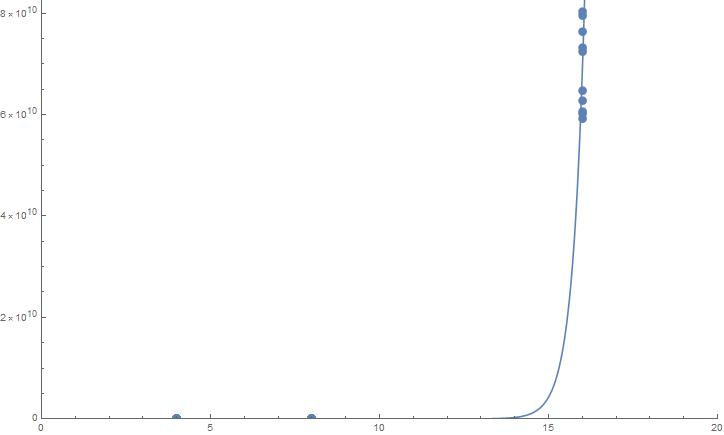
\includegraphics[scale=.5]{purebrute.jpg}\\
\centerline{number of inputs}


\centerline{\textbf{Increasing Random Brute Force}}
runttime 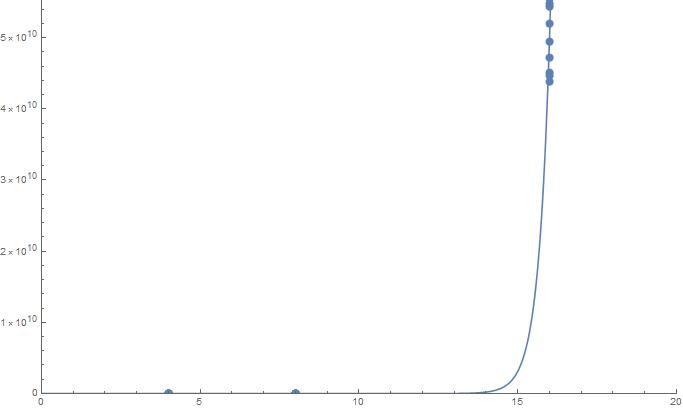
\includegraphics[scale=.5]{increasingbrute.jpg}\\
\centerline{number of inputs}
\\
\section*{Divide and Conquer}
\addcontentsline{toc}{section}{Divide and Conquer}
\ \\
To solve this problem from a divide and conquer approach, we 
bent the rules a little bit and utilized a \textit{decrease and conquer} 
technique we learned from Data Structures: the breadth first search 
technique. Rather than traversing every single permutation of a path like in 
the brute force solution, we recursively scan the graph breadth first to find
the optimal solution and return. Now rather than an worst 
case runtime of $O(V-1)!$ we now obtain a worst case runtime of $O(|V|+|E|)$.
This is misleading. Depending on the number of nodes you have this number can change.
We can either have $O(1)$ number of edges for a sparse graph or $O(V^2)$ for a
dense graph. Our real number of edges is somewhere greater than $O(V)$ and 
less than $O(V^2)$. The actual runtimes when we ran the simulations were 
clearly parabolic so the graph was assumed to be dense. This gives us a worst
case runtime of $O(V^2)$.
\\
Below we can see the experimental results for breadth first search. The runtime was
fitted to a model of $36002.6 V^2$ while the increasing order was 
fitted to $12902.7V^2$. From the graph a clear parabolic relationship
can be seen. In reality there are some $\log{V}$ and other $V$ terms giving
it the exact shape that it has but the parabolic term is clearly the dominating
one.\\\\
\newpage
\centerline{\textbf{Pure Random Breadth First Search}}
runtime 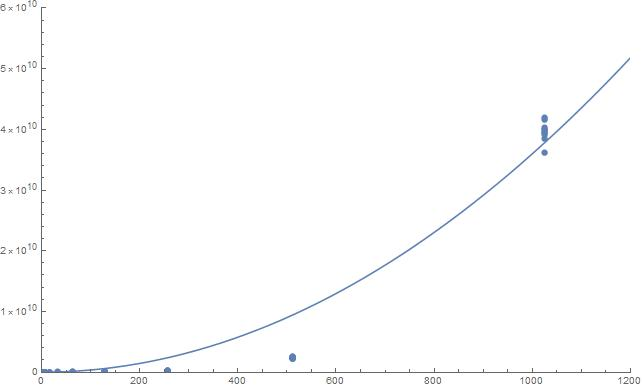
\includegraphics[scale=.5]{pureBFS.jpg}\\
\centerline{number of inputs}
\centerline{\textbf{Increasing Random Breadth First Search}}
runttime 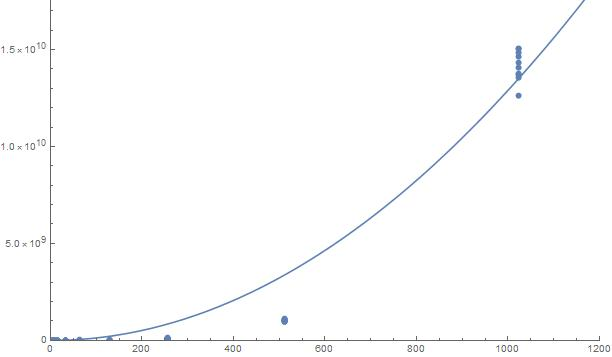
\includegraphics[scale=.5]{increasingbfs.jpg}\\
\centerline{number of inputs}
\\
\section*{Dijkstra's Algorithm}
\addcontentsline{toc}{section}{Dijkstra's Algorithm}
 \ \\
For the dynamic approach to this problem we will utilize Dijkstra's shortest 
path algorithm. The dynamic programming table is initialized first by taking 
care of the base cases (setting $R(i,i)=0$ and $R(i,j)=\infty$ if $i>j$) and 
setting the estimated "distance" to the rest of the vertices to infinity. Next 
using Dijkstra's algorithm we traverse the graph from vertex to vertex
the estimated infinity distances with the smallest edge weight sum that it
takes to traverse to that vertex. By filling in the smallest edge weights in
for vertex distances, we're also storing a partial solution to the answer that
we're looking for.\\\\
The asymptotic complexity of this algorithm is the same as breadth first search
: $O(|V|+|E|)$ and like breadth first search the complexity reduces down to:
 $O(|E|)$. For the same reasons discussed in the breadth first search section
 the runtime is $O(V^2)$. Given infinite time and more sleep a priority queue or
 fibonacci que would have been attempted but in the interest of my exam grades,
 the quickest solution that worked was implemented. The constants are clearly 
 smaller for Dijkstra's algorithm as opposed to breadth first search. Below 
 we can see the experimental results for Dijkstra's algorithm. The pure random runtime was
fitted to a model of $1486.33  V^2$ while the increasing order was 
fitted to $1482.97V^2$. From the graph a clear parabolic relationship
can be seen. In reality there are some $\log{V}$ and other $V$ terms giving
it the exact shape that it has but the parabolic term is clearly the dominating
one.
 \newpage
 \centerline{\textbf{Pure Random Dijkstra's Algorithmh}}
 runtime 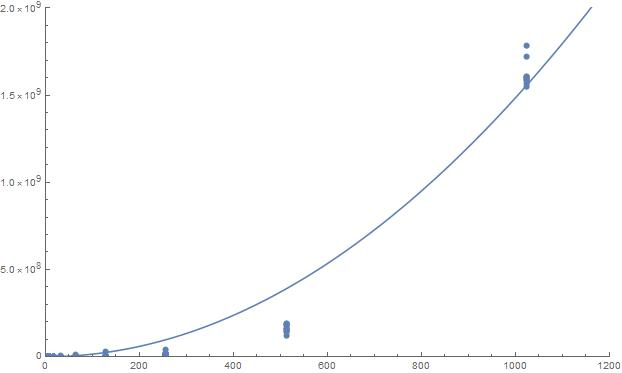
\includegraphics[scale=.5]{puredij.jpg}\\
 \centerline{number of inputs}
 \centerline{\textbf{Increasing Random Dijkstra's Algorithm}}
 runttime 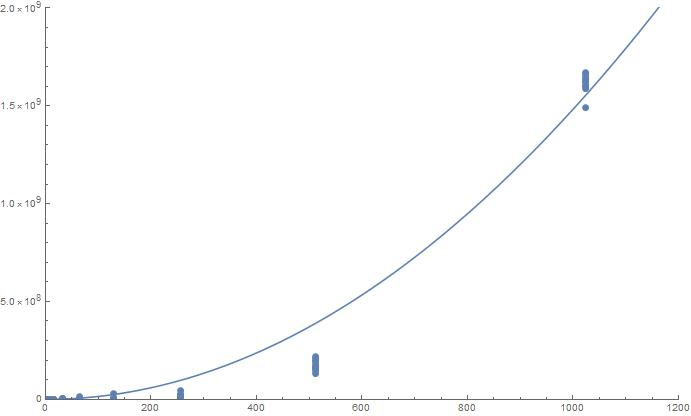
\includegraphics[scale=.5]{incdij.jpg}\\
 \centerline{number of inputs}
 \newpage
 \section*{Conclusion}
 \addcontentsline{toc}{section}{Conclusion}
The runtime between BFS and Dijkstra's algorithm is a full factor of ten less.
While they are asymptotic to each other, this is worth knowing in practice. It
is also worth noting that the constants essentially stay the same for Dijkstra
depending on the different inputs. This would to me make me think that Dijkstra's
algorithm is better than BFS for solving this problem. Not only is it faster by a factor
of ten but is is more reliable. As Knuth says, an algorithm must be seen to be believed.
All group members worked on this project but a majority of the graph construction
and algorithm implementation was completed by Jake. Dijkstra's A Discipline of Programming
changed Jake's life. He read it four years ago while he was a political science
student and decided that he wanted to move the entire distance across America 
and study Computer Engineering at the University of Washington. It was a pleasure
to finally implement Dijkstra's algorithm. It's been a long road to get to this
point, and he didn't take the shortest path, but the destination was finally found.
Thank you for this quarter and I'll see you in the fall.  
%-------------------------------------------------------------------------------
% REFERENCES
%-------------------------------------------------------------------------------
\newpage
\section*{References}
\addcontentsline{toc}{section}{References}
\url{https://youtu.be/i_AQT_XfvD8?t=22m15s}
\newline
\newline
\url{https://www.coursera.org/lecture/advanced-algorithms-and-complexity/brute-force-search-x60TX }
\newline
\newline
\url{http://www.cs.cmu.edu/afs/cs/academic/class/15210-f12/www/lectures/lecture10.pdf}
\newline
\newline
\url{https://ocw.mit.edu/courses/electrical-engineering-and-computer-science/6-046j-design-and-analysis-of-algorithms-spring-2012/lecture-notes/MIT6_046JS12_lec06.pdf}
\newline
\newline
\url{https://www.geeksforgeeks.org/decrease-and-conquer/}
\newline
\newline
\url{http://www.csl.mtu.edu/cs4321/www/Lectures/Lecture\%2010\%20-\%20Decrease\%20and\%20Conquer\%20Sorts\%20and\%20Graph\%20Searches.htm}
\newline
\newline
\url{https://ocw.mit.edu/courses/electrical-engineering-and-computer-science/6-046j-design-and-analysis-of-algorithms-spring-2012/lecture-notes/MIT6_046JS12_lec06.pdf}
\newline
\newline
\url{https://youtu.be/NzgFUwOaoIw?t=15m20s}
\newline
\newline
\url{https://winterbe.com/posts/2014/07/31/java8-stream-tutorial-examples/}
\end{document}
